\documentclass[]{article}

%\usepackage{cogsci}
\usepackage{pslatex}
\usepackage{apacite}
\usepackage{graphicx}
\usepackage{booktabs,caption,fixltx2e}
\usepackage{rotating}
\usepackage[letterpaper, margin=1in]{geometry}

\usepackage{pdflscape}

%opening
\title{Delay d'ETRE: Explict Temporal Ratios Lead to Impatience}
\author{Daniel Wall}


\begin{document}

\maketitle

\begin{abstract}
	When selecting a shipping speed on Amazon we are faced with a choice between getting our package sooner but paying more money, or getting our package later and paying less money. 
	The general phenomenon underlying our expedited shipping is impatience, we want good things immediately and we must be compensated for waiting. 
	Previous research on intertemporal framing has shown that displaying times as dates -- January 23rd -- as opposed to delays -- 6 weeks -- increases patience. 
	Other research has shown that people use both differences and ratios of time in intertemporal choices. 
%	These two results suggest that framing times as ratios alters patience. 
%	In three experiments I manipulate the temporal presentation from the standard -- 1 day versus 5 days --  to making the ratio explicit -- 1 day or 5 times as long.  
	Across three experiments I show that making temporal ratios explict leads to differing levels to increase impatience in standard  intertemporal choices framed as gains, intertemporal choices framed as losses, and for an explicit shipping scenario. 
	Taken together these results suggest that framing delays as ratios leads to greater impatience.
	 
%
%	People use ratios in everyday life -- intertemporal choices are no different, 
%	recent cognitive models of intertemporal choice show that people calculate ratios of both money and time. 
%	These models account for diminishing impatience -- when items are moved into the future, people are more patient. 
%	Our goal is twofold: 1) to show that previous models of intertemporal choice do not properly account for temporal ratios and present a conceptual model of time discounting, and  2) by explicitly manipulating how people use ratios of time, we can alter how people make intertemporal choices. 
%	This leads to novel predictions for how to optimally frame intertemporal choices to induce either patience or impatience. 
%	Further we show that in a hypothetical shipping scenario that when temporal ratios are explicit, people are more impatient. 
	
\end{abstract}

\section{Introduction}

All of us have felt the itch to get the new purchase we made on Amazon as quickly as possible; sometimes leading us choosing expedited shipping, even at considerable cost. 
Generally on Amazon we see shipping times as the number of days until you will receive your package, e.g.  ``Receive your package in 2 days''. 
The shipping time could also be described as ``Receive your package on December 17th''. 
This reframing of delays -- 2 days -- into dates -- December 17th -- has been shown to increase patience \cite{Read2005}.
Occasionally Amazon frames shipping times as dates, possibly to induce customers to be more patient and receive their items later. 

However a firm may want consumers to be impatient and choose the expedited shipping option. 
If a firm's inventory is high they may want to nudge consumers to ship their items faster. 
It is important to understand what variables consumers are using and how they are making intertemporal choices to create robust and adaptive choice environments. 
This understanding how to optimally display information leads to novel predictions for how to frame shipping speeds. 

How the monetary and temporal aspects of an intertemporal choice are framed lead to varying degrees of patience.
Further, recent models of intertemporal choice have posited that people use ratios in intertemporal choices \cite{Read2013, MarzilliEricson2015}. 
%For instance \citeA{Read2013} found that by making ratios in the 
However, to the best of my knowledge, no study has investigated how explicitly framing time as a ratio can alter patience.
Further although shipping scenarios are a form of intertemporal choice, they differ from how most studies operationalize intertemporal choices. 
Across 3 studies I show that by making ratios explicit people are more impatient in intertemporal choices. 
%Further we show that by making the ratios between times explicit we can induce a higher reliance on ratios.
This result holds for intertemporal choices framed as gains, losses, and in an explicit shipping scenario. 
As opposed to other studies which showed that reframed times as dates increases patience, framing times as ratios decreases patience.
Firms wanting to decrease patience in their consumers may want to frame intertemporal choices as ratios as opposed to delays.
 

%If the temporal ratio is explicit people are more impatient than when the ratio is implicit.



%
%There are subtle ways in which the presentation of time can alter patience. 
%For instance people are more impatient when delays are calendar dates as opposed to delays into the future \cite{Read2005}. 
%Marketers have used temporal frames in shipping scenarios.
%For example as opposed to stating that you will receive your package in 2 weeks, Amazon sometimes states that you receive your package on January 23rd. 
%As per \citeA{Read2005} this frame will increase patience. 

%Many of our daily choices involve making decisions involving time in some respect, often taking the form of a the tradeoff between receiving something of smaller value now and receiving something of larger value in the future. 
%For instance when a consumer selects a shipping speed when shopping online they are making an intertemporal choice.
%These decisions require consumers to, perhaps implicitly, calculate how much waiting for the slower shipping speed is worth.  

%Firms could, however, prefer that a consumer is impatient when choosing a shipping speed. 
%If a firm's inventory is low on a particular item they may not profit from the extra cost that it takes to expedite shipping, however if their inventory is high they may want to nudge consumers to ship their items faster. 
%It is important to understand what variables consumers are using and how they are making intertemporal choices to create robust and adaptive choice environments. 
%This understanding how to optimally display information leads to novel predictions for how to frame shipping speeds. 
%
%Recent models of intertemporal choice have posited that people use ratios in intertemporal choices [ITCH, DRIFT]. 
%Across [] studies we show that how people make intertemporal choices is dependent on how they perceive ratios. 
%Further we show that by making the ratios between times explicit we can induce a higher reliance on ratios. 
%If the temporal ratio is explicit people are more impatient than when the ratio is implicit.

\section{Literature Review}

Intertemporal preferences measured in marketing and psychology are generally studied by choices between a smaller sooner and larger later amounts of money \cite{Zauberman2014}. 
There are four general categories of research on  intertemporal choices (see \citeA{Read2013} for an overview).
The first focuses on how magnitude of both time and money effects patience \cite{Scholten2006, Thaler1981}
the current paper belongs to research investigating how patience is altered by option frames. 
The second stream focuses on how choices relate to real world behavior.
Individual differences in imputed discount functions predict real world phenomenon such as credit card debt,  mortgage choice, and smoking \cite{MacKillop2011, Meier2009, Johnson2011}. 
The third stream focuses on how emotional states can alter intertmporal preferences, e.g. being shown freshly baked bread \cite{Li2008}. 
The fourth stream investigates how the framing of options affects patience. 

An example of option framing in intertemporal choice is the hidden zero effect -- when the implicit zeros in intertemporal choices are made explicit people are more patient \cite{Magen2008}. 
For instance when a choice between ``receiving \$100 now'' and ``\$110 in 6 months'' is reframed to be  ``receiving \$100 now \textit{and nothing in six months}'' and ``\$110 in 6 months \textit{and nothing now}'' people are more patient. 

Additionally \citeA{Read2013} show that making the ratio between amounts salient affects intertemporal choices. 
Specifically when the magnitude of amounts is small, reframing the amounts as interest rates leads to increased patience. Taking the above example, when reframed as an interest rate, e.g.  a choice between  ``receive \$100 now'' and ``receive 10\% more in six months'' people are more patient. \citeA{Read2013} posit that interest framed amounts lead to an increased reliance on ratios of monetary amounts.

Beyond amounts, times can also be reframed.
The most famous example of temporal reframing is  Lincoln's Gettysburg Address which made 87 years into the ``Four score and seven years ago''.
\citeA{Read2005} shows that how a times are framed in intertemporal choices can alter patience. 
Taking the above example, people are more patient when reframed it as a choice between  ``receive \$100 now'' and ``receive \$110 on June 15'' -- this is known as the delay/date effect. 
The delay/date effect demonstrates that perceived temporal distance is dependent on how delays are framed. 

In other work on intertemporal choices, \citeA{MarzilliEricson2015} show that in intertemporal choices framed as ``receiving \$100 now'' and ``\$110 in 6 months'', people rely on both differences and ratios of the  attributes of intertemporal choices -- monetary amounts and times.
Their model -- the Intertemporal Choice Heuristic (ITCH) -- does better at predicting intertemporal choices than classic models, such as hyperbolic or exponential discounting. 
As seen in Equation~\ref{eq:itch}  the functional form of the ITCH model with estimated parameters shows that an increased reliance on ratios in time leads to steeper discounting. 

[What are they?]
 
 \begin{equation}\label{eq:itch}
 P(LL) = L \left(\beta_I + \beta_{xA}(x_2 - x_1) + \beta_{xR} \frac{x_2 - x_1}{x^*} + \beta_{tA}(t_2 - t_1) + \beta_{tR} \frac{t_2 - t_1}{t^*}\right)
 \end{equation}
 
 
This work aims to demonstrate that the fourth research stream -- that patience is affected by how options are framed -- can affect real world phenomenon.
Specifically, this paper combines the work of \citeA{Read2013} -- which shows that framing amounts as ratios alters patience -- and \citeA{MarzilliEricson2015} -- which shows that people rely on differences and ratios in standard intertemporal frame as well as the work  of  \citeA{Read2005} which shows that how times are framed can alter patience. 

Specifically, I focus on how framing times as ratios can decrease patience.
When delays are sufficiently small, and when temporal ratios are made explicit, our attention will be focused on the ratio of how much \textit{longer} we will wait. 
For instance reframing a choice between ``receiving \$100  in 1 day'' and ``\$110 in 10 days'' to being a choice between ``receiving \$100  in 1 day'' and ``\$110 in 10 \textit{times as long}'', will focus participants on how much longer they will wait for \$110 as opposed to receiving the \$100 today.
This increased focus on how long they will wait, leads to decreased patience when times are framed as ratios.

\subsection{Hypothesis}

\subsubsection{Hypothesis 1}
Given that people rely on differences and ratios between amounts and times in intertemporal choice, increasing the reliance on ratios for times with relatively small differences should lead to decreased patience.

\textit{Hypothesis 1:} In gain intertemporal choices, when times are expressed as ratios, people will be more impatient than when expressed as delays. 

\subsubsection{Hypothesis 2}
Similar to hypothesis 1 when framed as losses making temporal ratios explicit people will be more impatient. 

\textit{Hypothesis 2:} In loss intertemporal choices, when times are expressed as ratios, people will be more impatient than when expressed as delays. 


\subsubsection{Hypothesis 3}
Related to hypothesis 2 when framed an intertemporal chioce is framed as a shipping scenario,  making temporal ratios explicit people will induce less patience. 

\textit{Hypothesis 3:} In shipping scenarios, when times are expressed as ratios, people will be more impatient than when expressed as delays. 


\subsection{Summary of Studies}

In this paper, I describe three studies investigating the explicit temporal ratio effect (ETRE).
Study 1 shows that the explicit temporal ratios lead to less patience when intertemporal choices are framed as gains.
Study 2 extends this effect to losses.
Finally, Study 3 shows that in an explicit shipping scenario people are less patient when temporal ratios are made explicit. 

 

%Study 2 extends the results of Study 1 to losses. 
%Although most intertemporal choice studies use gains, a large number of real world intertemporal choices involve losses \cite{Hardisty2013}. 
%For instance waiting to pay off your credit card incurs greater losses if you wait -- the compounding interest -- than if pay it off immediately.
%Intertemporal choices framed as lossed measured in the lab take the form of choices between ``Pay \$100 immediately'' and  ``Pay \$110 in 6 months'' \cite{Hardisty2015}.
%Further most studies investigating framing effects on intertemporal choices are restricted to the domain of gains. 
%Study 2 investigates how framing times as ratios leads to decreased patience in losses. 
%
%Study 3 extends the results from Study 1 and Study 2 to intertemporal choices explicitly framed as shipping scenarios.
%Shipping scenarios are typically displayed as a choice between ``Receive your items in 2 days and pay \$8'' and ``Receive your items in 10 days and pay \$4''
%Although choosing a shipping speed is similar to the previous intertemporal choices there is a subtle, yet possibly significant difference between the two.
%Shipping decisions can be thought of as \textit{paying more now to receive an item sooner} whereas the intertemporal choices shown in Study 2 can be thought of as \textit{paying something smaller now to avoid paying something larger later}.
%This difference in choices  
%



\section{Study 1}
Study 1 shows that the explicit temporal ratios lead to less patience when intertemporal choices are framed as gains.
Participants chose between smaller sooner and larger later options. 
These options were displayed in one of two frames: implicit temporal ratios and explicit temporal ratios. 
Study 1 tests Hypothesis 1: In gain intertemporal choices, when times are expressed as ratios, people will be more impatient than when expressed as delays. 

\subsection{Method}
Two hundred participants from Amazon Mechanical turk we recruited to take part in a ``Decision Making Survey''. 
Although the validity of Mechanical Turk has been called into question, \citeA{Paolacci2010} finds that classic effects in decision making replicate. 
Further, participants who have less than 50 HITs accepted or  who have less than 95\% of their HITs accepted were not allowed to participate in the study. 
Additionally only participants who passed an attention check were included in the final analysis.
These precautions were taken to ensure that participants were paying attention to the study 

Participants completed informed consent, then were given a test to ensure they understood the paradigm.
Next they were assigned to one of the two conditions: implicit ratio or explicit ratio. 
They then were shown the five intertemporal choices in from the Study 1 section of  Table~\ref{tab:stimuli}. 
Choices were displayed in a randomized order


\begin{landscape}
\begin{table}[!ht]
	\caption{Amounts and times of Stimuli for Studies 1-3} 
	\label{tab:stimuli}
	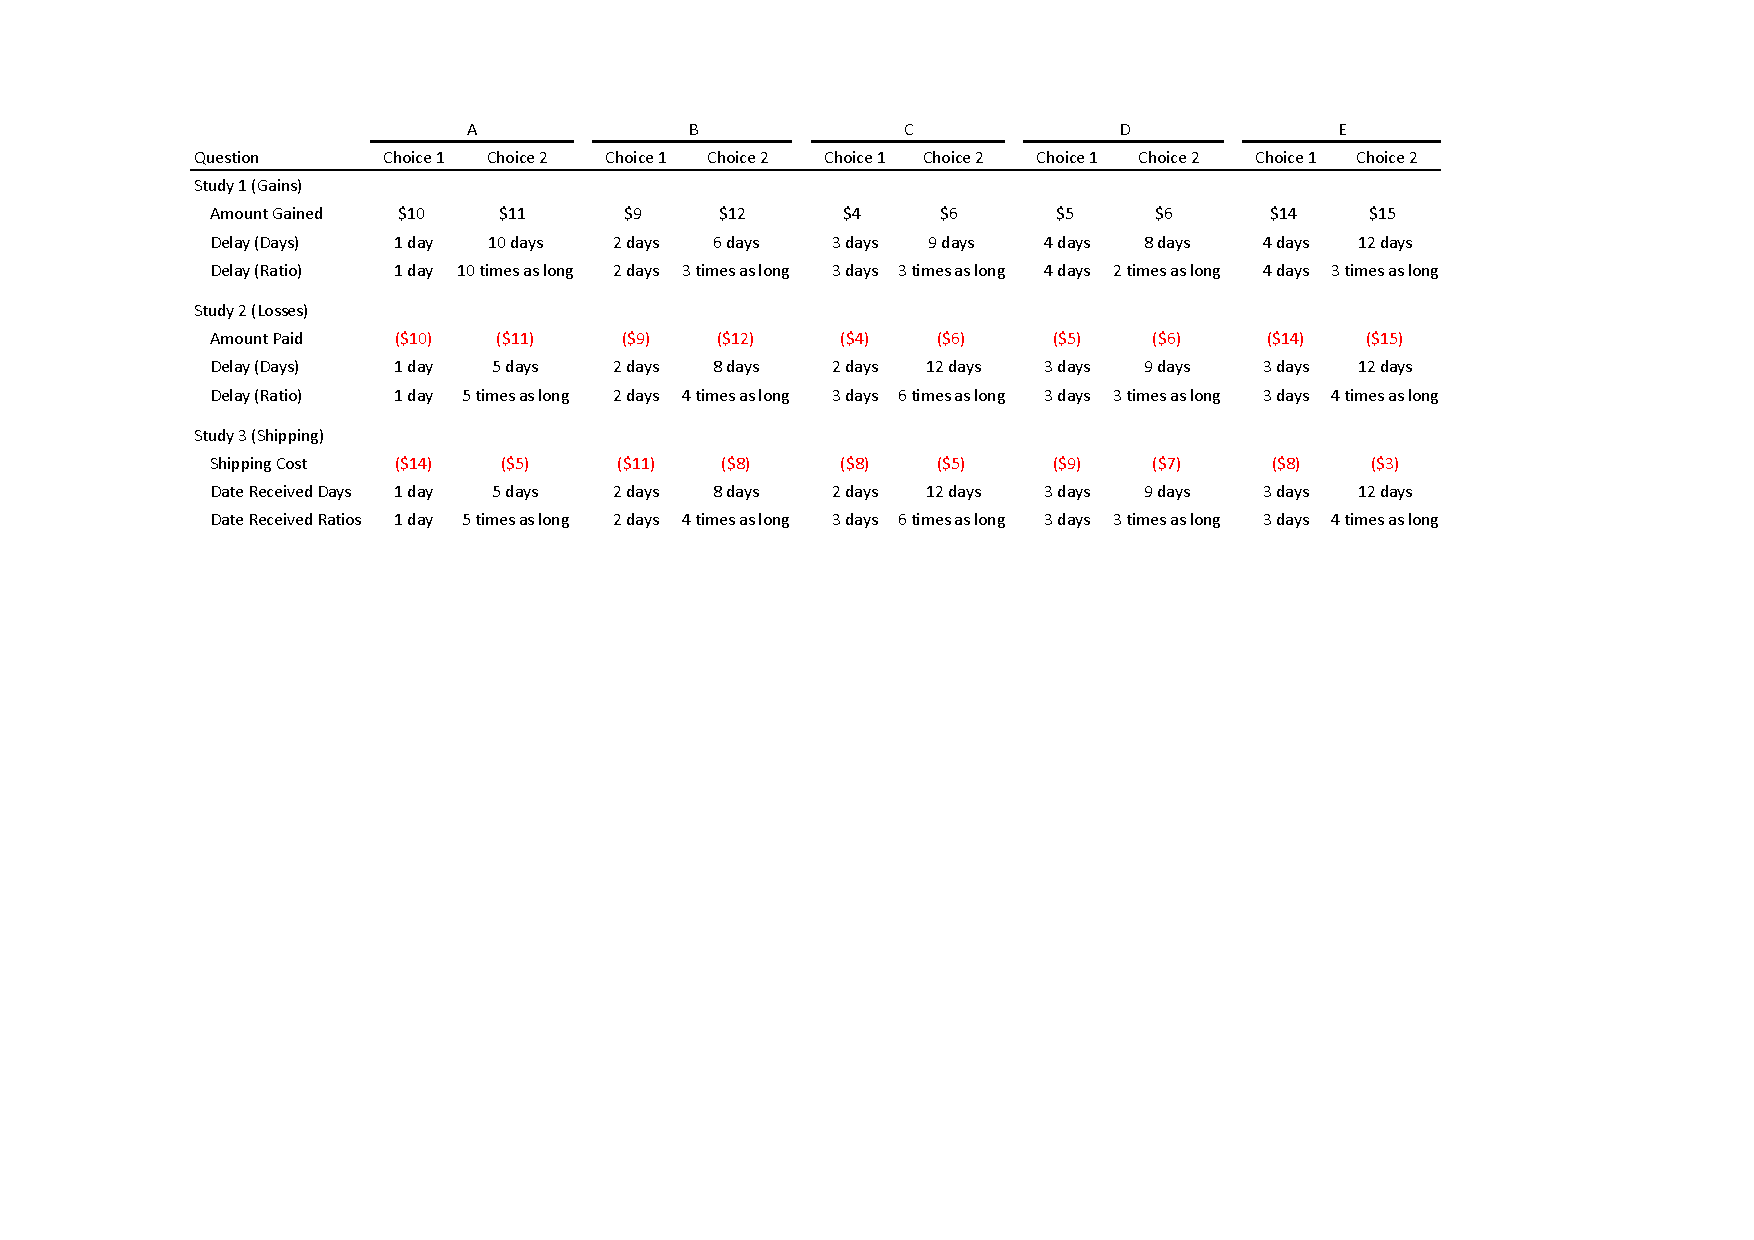
\includegraphics[]{Stimuli_For_Study.pdf}
\end{table}
\end{landscape}

For the implicit time ratio condition, intertemporal choice A was displayed as follows: 

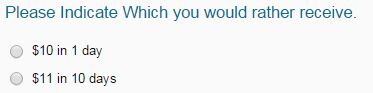
\includegraphics[]{study1_implicit}

Choices B-E were displayed in the identical format. 

In the explicit time ratio condition, intertemporal choice A was displayed as follows:

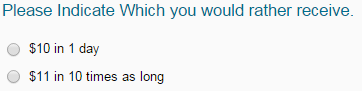
\includegraphics[]{study1_explicit}

Choices B-E were displayed in the identical format. 

Further each choice was displayed in a random order to each participant. 
After completing their choices participants completed demographic information.

\subsection{Results}

Following \citeA{Read2005} and \citeA{Hardisty2015}, the dependent variable was the number of times the participant chose sooner reward (option 1 in Table~\ref{tab:stimuli}). 
As seen the Table~\ref{tab:study1results} (note I did not actually collect data for this study I just put sample data down for illustrative purposes) there is a strong effect of explicit intertemporal ratios. 
Nearly twice as many people choose the sooner option when temporal ratios are explicit.




\begin{table}[!ht]
	\caption{Proposed Percent of choices for the sooner option given different temporal ratios} 
	\label{tab:study1results}
\begin{tabular}{ p{3cm}||p{3cm}|p{3cm}  }
	\multicolumn{3}{|c|}{Temporal Frame} \\
	\hline
	 & Implict Ratio & Explicit Ratio\\
	\hline
	A (\%)	 & 30  & 60\\
	B (\%) 	 & 40  & 65   \\
	C (\%) 	 & 42  & 70\\
	D (\%)   & 37  & 68\\
	E (\%)   & 39  & 66\\
	Mean (\%) & 38  & 65.8 \\
	N  	 & 100  & 100\\
	\hline
	
\end{tabular}
\end{table}

Statistical significance of  the difference between explicit and implicit temporal ratios was tested via a Kruskal-Wallis tests.
 Overall the effect of ratio was significant. 
 To confirm these results, I ran a robust logistic regression which allowed for correlated errors within participants.
 The dependent variable was choice (0 later option chosen, 1 sooner option chosen) and the independent variable was ratio frame. 
 This regression confirmed the results of the Kruskal-Wallis test, namely that participants were more impatient when temporal ratios are make explicit. 
 

\section{Study 2}


\section{oldstuff}


Ratios are ubiquitous in the modern world and are paramount in disparate fields from the stock market to baking. 
When making inferences from ratios, people are biased in predictable ways.
For instance, Yamagishi showed that ratios with large numerators and denominators are perceived to be riskier than ratios with small numerators and denominators. Further, Reyna and Brainerd argued that people overweight numerators compared to denominators.
The biases used when calculating ratios are relevant to intertemporal choices. 

Recent models of intertemporal choice have posited that people use ratios to decide between a smaller sooner and a larger later option [ITCH, DRIFT]. 
An example intertemporal choice is choosing between \$5 in 1 day and \$6 in 5 days. 
The ITCH model would predict that participants calculate differences between and ratios of both the dollar amounts and the times. 
If people are biased in calculating ratios for everyday items, it follows that they would be biased in calculating ratios in intertemporal choices. 

One of the empirical regularities in intertemporal choice research is that impatience decreases when times are moved away from the present.
If we took the above example and moved both options back by 20 days we would see more patient responses. 
Multiple explanations for this phenomenon -- known as decreasing impatience -- have been marshaled. 

Zauberman showed that taking into account subjective perceptions of time can account for decreasing impatience. 
For instance they find that the subjective time perception of 1 year is not different from the subjective time perception of 3 years. 
Further subjective time perception was shown to follow a psychophysical logarithmic function. Zauberman, however, embedded this subjective time perception into a hyperbolic discounting function – an alternative based discounting function.  

Beyond accounting for diminishing impatience subjective time perception can account for subadditive discounting. 
Read (2001) found that intertemporal choices are intransitive, specifically “discounting over a delay is greater when the delay is divided into subintervals than when it is left undivided”. 
However, Zauberman showed that participants perceive the total time horizon as longer when it is divided into subintervals than when it is not divided. 
Further participants discounted more when the delay was divided into subintervals than when it was undivided. 

The focus of this paper is on how people calculate ratios specifically about time. 
We hypothesize that the ratio change in times alters the extent of decreasing impatience. 
We begin with a review of the current discounting models and how they account for decreasing impatience. 
Further we will show that while some models predict that ratio change will have an effect on decreasing impatience, that none of the models predict effects as large as we see. 
These results introduce a phenomenon whose extent is not captured by the current discounting models. 
They show that the properties of the numbers given can alter patience via their ratio. 
Moreover recent models of intertemporal choice do not properly predict the degree of decreasing impatience properly, we show that our modification to their model does a better job of predicting choices. 

We then apply our conceptual model to situations where temporal ratios are explicit. 


\section{Discounting Models}

When presented with a choice between receiving A) \$10 in 5 days or receiving B) \$12 in 7 days, there are a large number of calculations you could perform to decide which to choose.  Alternative based theories -- such as exponential and hyperbolic discounting -- posit that you calculate a discounted utility for each option. Whereas other, attribute based models, posit that people make comparisons attribute based comparisons -- they compare the money and time amounts to one another. 

\subsection{Exponential Discounting}

The normative model of intertemporal choice is exponential discounting.
The exponential discounting function is  

\begin{equation}\label{eq:exp}
	\delta_{exp} = \exp^{-rt}
\end{equation}


Where $\delta$ is the discount fraction which each monetary amount is multiplied by and $r$ is the exponential discount rate. And the utility of an option is:

\begin{equation}\label{eq:utilalt}
	U(x, t) = x \delta
\end{equation}



 If the daily exponential discount rate is .01 then the current value of A) Would be $\$10 * \exp^{-.01*5} = 9.5$ and the current value of B) would be $\$12 * \exp^{-.01*7} = 11.19$

From \cite{@Toubia2014} Toubia 2014 we can get the probability of choosing larger later from the following formula

\begin{equation}\label{eq:pll}
	P_{LL} = \frac{\exp(U_{LL})}{\exp(U_{LL})+ \exp(U_{SS})}
\end{equation}


Using this formula we get the following probability of choosing larger later $\frac{11.19}{11.19+9.5} = .54$

One of the empirical regularities in intertemporal choice research is that impatience decreases when times are moved away from the present. The exponential model, however, does not account for this phenomenon. For instance if we added 100 days to both A and B yeilding C) \$10 in 105 days and D) \$ 12 in 107 days the utility of C would be $3.5$ and the utility of D would be $4.11$. Plugging into equation \ref{eq:pll} we get $.54$, the same answer we saw before. 

\subsection{Hyperbolic}

Hyperbolic discounting has been shown to account for decreasing impatience

\begin{equation}\label{eq:hyp}
\delta_{hyp} = \frac{1}{1+kt}
\end{equation}

Where $k$ is the hyperbolic discount rate, and the utility of the option is found by equation \ref{eq:utilalt}.

Assuming daily $k = .01$, for choice A) \ref{eq:hyp} we get $\delta_A = \frac{1}{1+.01*5} = .952$ meaning the utility is $9.52$ and for B) the utility is $11.21$ which yields a larger later probability of $.541$. When we look at the larger later probabilities for C and D we get, 4.88 and  5.79 yielding a larger later value of $.543$. There's an increase in the likelihood of choosing the larger later option when both options are moved into the future, this is known as diminishing impatience. 

The hyperbolic and exponential models both predict that people make alternative based transitions; however recent models have shown that people make attribute based transitions



\subsubsection{Subjective Time Perception}

Zauberman showed that peoples subjective perception of time can account for hyperbolic discounting. 

\subsection{ITCH}
\label{ITCH}

Marzilli Ericson and colleagues showed that fully attribute based models can predict out of sample choices better than alternative based models. 
According to ITCH the probability of choosing larger later is

%\begin{equation}\label{eq:itch}
%	P(LL) = L \left(\beta_I + \beta_{xA}(x_2 - x_1) + \beta_{xR} \frac{x_2 - x_1}{x^*} + \beta_{tA}(t_2 - t_1) + \beta_{tR} \frac{t_2 - t_1}{t^*}\right)
%\end{equation}

In the paper they give the example parameters for each of the coefficients of 0, .1, .1. -.1, -.1. Using these coefficients in equation \ref{eq:itch} for A compared to B the probability of choosing larger later would be $.496$, whereas for C and D the probability of choosing larger later would be $.504$


\subsection{Discounting By Intervals}

\begin{equation}\label{eq:int}
	D(t_S, t_L) = \left(1 + \alpha \left(\frac{w(t_L) - w(t_S)}{\vartheta}\right)^{\vartheta}\right)^{-\beta/\alpha}
\end{equation}


\subsection{Trade-off model}

% %\begin{equation}
% %Q(w(t_L) - w(t_S)) = 
% %\begin{cases}
% %v(x_L) - v(x_S), & \text{if}\ x_L > x_S > 0 \\
% %v(x_S) - v(x_L), & \text{if}\ 0 > x_S > x_L
% %\end{cases}
% %\end{equation}

\subsection{Summary}
Taken together these models show that some models predict that a large ratio change will have more decreasing impatience than a small ratio change; however we posit that the degree of  decreasing impatience will be larger when the ratio change is small compared to when it is large.
Take the following two choices for example $SS_{sr}$ = \$10 in 5 days and $LL_{sr}$ = \$12 in 6 days and $SS_{lr}$ = \$10 in 5 days and $LL_{lr}$ = \$12 in 10 days. Where $SS_{sr}$ stands for the smaller sooner option for the small time ratio. 
If we add 5 days to both items they would now be $SS_{sr}^{del}$ = \$10 in 10 days and $LL_{sr}^{del}$ = \$12 in 11 days and $SS_{lr}^{del}$ = \$10 in 10 days and $LL_{lr}^{del}$ = \$12 in 15 days. 

[Insert a table about the degree of decreasing impatience for each model here]

\section{Time Ratio Model (TRaM)}

We propose a new model of ITC which can account for the degree of decreasing impatience based on the ratios of time. 
We begin with a verbal description of our model

\subsection{An example of TRaM}

When presented with a choice between \$5 in 1 day and \$10 in 5 days. 
A TRM decision maker would look at the two delays and calcluate their ratio. 
Then they will use a rule of thumb to say how much relative compensation they need to account for that ratio.
Below is an example of a TRM decision maker would make an intertemporal choice:

The time is 5 times as long therefore I will need about 3 times as much money. 

If people use this heuristic then the ratio between times becomes important. 
If we move both options up by five days then the ratio between times becomes $10/6$ = 1.66. A participant using the TRM heuristic would say that 
The larger later time is about 1.5 times as long as the smaller sooner time therefore I need about 1.25 times as much money. 

Further TRaM predicts that the salience of the temporal ratio means that it is more likely to be used. 
For instance if the temporal ratio explicit, participants reliance on it would increase.



\section{Combining ITCH, DRIFT, and TRaM }

Read, Frederick, and Scholten (2013) show that when making intertemporal choices how the monetary amounts are framed alters patience. 
They propose a Difference, Ratio, Interest, Finance, and Time (DRIFT) model of intertemporal choice. 
For instance when an intertemporal choice is framed as \$100 now OR \$110 in 1 year people will rely on differences in monetary amounts.
However if the choice is framed as \$100 now or an extra 10 \% after 1 year, people will rely more on ratios. 
The DRIFT model of intertemporal choice shows that how monetary amounts are framed can alter levels of patience.

Relatedly Read, Frederick, Orsel, and Rahman showed that how the times intertemporal choice are displayed can affect patience. Specifically Read and colleagues found that when times are described as dates (e.g. December 30th) people are more patient than when described as delays (e.g. in 1 month). Temporal framing can alter patience. 

Given that temporal framing can alter patience and that people rely on ratiosin intertemporal choice, we propose that making ratios between times explicit can alter patience. 
For instance, an intertemporal choice between receiving \$10 in 2 days and \$11 in 12 days could be re-framed as \$10 in 2 days and \$11 in 6 times as long. 
We proposed that this temporal framing leads to a greater weight being placed upon the time ratio term $\beta_{tR}$ and a lower weight on the time difference term $\beta_{tA}$ in equation \ref{eq:itch} . Taking the example and using the parameters in section \ref{ITCH} the probability of choosing larger later is $.26$. However if the ratio is weighted more heavily -- the absolute value of the beta coefficient goes up e.g.  $\beta_{tR} = -.5 $ -- and the difference is weighted the same, eg. $\beta_{tA} = -.1$, the probability of choosing larger later is now $.0065$. 

Holding everything else constant by making the temporal ratio more salient, e.g. increasing the absolute value of $\beta_{tR}$,  monotonically decreases the probability of choosing larger later. We propose that making temporal ratios more salient increases their decision weight, leading to more impatient choices

{\large [This CANNOT account for the change in the decision weight on temporal differences by making temporal ratios salient, which I am unsure of how to work out]. 
}

The TRaM conceptual model of intertemporal choice suggests that by making temporal ratios explicit that people's reliance on them will be higher.
When people's reliance on temporal ratios is higher, the weight in which temporal ratios receive will be higher. 
This weight has predictable consequences on how impatient participants are, which suggests ways in which firms can alter patience based on how times are presented. 




\section{Study 1}

In study 1 we will test this prediction of the degree of decreasing impatience depending on the change in ratio.
We predict that when ratio changes are large, participants will show more diminishing impatience than when ratio changes are small. 

\subsection{Methods}
Participants were in one of two conditions. 
Six intertemporal choices were consistent across conditions and were used to calculate the participants discount fraction.
The other two intertemporal choices varied across conditions, these choices varied in the extent to which the temporal ratio changed.
We varied the ratio with either a small or large time ratio which was moved into the future by 5 days. 

In condition 1 participants the two focal questions were:  
\$10 in 5 days or \$11 in 6 days
and 
\$10 in 10 days or \$11 in 11 days

In condition 2 participants the two focal questions were: 
\$10 in 5 days or \$11 in 15 days
and 
\$10 in 10 days or \$11 in 20 days

In condition 1 the change in temporal ratio is small (1.2 to 1.1), whereas in condition 2 the change in temporal ratio is large (3 to 2). 


\subsubsection{Participants}

We recruited [] Rutgers university undergraduates to complete the study for course credit. 

\subsection{Results}
 
We calculated the daily discount fraction for each of the four focal items while controlling for the participants discount fraction from the other 6 items. 
The degree of decreasing impatience was calculated by taking the difference between the daily discount fraction from the two focal items. 
We ran a multilevel linear regression predicting the degree of decreasing impatience with condition and discount fraction of the other items as predictors. 

The regression showed that the degree of decreasing impatience was predicted by condition.  

\subsection{Discussion}

Study 1 shows that the use of temporal ratios is more important than other cognitive models predicted. 
If temporal ratios are important, by explicitly manipulating them, we should be able to alter levels of patience

\section{Study 2}

In study 2 we manipulate how easy it is to compare temporal ratios. 
From ITCH and TRaM we hypothesize that participants who are shown explicit temporal ratios will make more impatient decisions 

\subsection{Methods}

Each respondent answered 27 questions framed as intertemporal choices.
We varied the time to the smaller sooner option ($SS_{time} =$ 5, 10, or 50 days), 
the ratio between the smaller sooner and larger later times ($SS_{time} / LL_{time}  = $ 1.2, 2.2, or 3.2 times as long), 
 the difference between the smaller sooner and larger later amount ($LL_{amnt} - SS_{amnt} =$ \$5, \$10, \$30). All smaller sooner amounts were \$47 [Or we could pull from a uniform distribution?].

Each respondent was assigned to one of two frames: implicit temporal ratios and explicit temporal ratios. An example of both is given below

\textbf{Implicit Temporal Ratio: } You can receive \$47 in 5 days or \$54 in 6 days

\textbf{Explicit Temporal Ratio: } You can receive \$47 in 5 days or \$54 in 1.2 times as long

\subsection{Results}

We perform a multilevel logistic regression predicting choice with varying intercepts for each participant, the three within subject factors, and the between subject factor of temporal ratio frame. 

The results of the logistic regression are shown in table []. We see that participants in the explicit temporal ratio are more impatient frame than those in the implicit temporal ratio frame. [Is there an interesting interaction here e.g. we see this effect only when the ratio is large but not when it is small?]


\section{Study 3}

While study 2 showed that when time ratios are explicit, people are more impatient, it was framed as gains not losses.
Most shipping situations involve a cost to the consumer. 
In Study 3 we replicate study 2 but with losses.

\subsection{Methods}

The methods for study 3 are identical to study 2 except that all monetary amounts are framed as losses and not gains. 

\subsection{Results}

We replicate the findings of study 2 when framed as losses. 

\section{Study 4}

Studies 1 and 2 showed that explicit time ratios make people more impatient for both gains and losses, but do not specifically deal with a shipping scenario. Study 4 uses a hypothetical shipping scenario.

\subsection{Methods}

Participants were told to imagine that they had just decided to buy \$75 worth of merchandise on a popular on-line vendor. 
[Should this strictly be between subjects?]

They then were presented with two shipping options in one of the two frames.

\textbf{Implicit Temporal Ratio}

Option 1: Receive your order in two days for \$7

Option 2: Receive your order in 10 days for \$3
 
 
\textbf{Explicit Temporal Ratio}

Option 1: Receive your order in two days for \$7

Option 2: Receive your order in 5 times longer than option 1 for \$3

\subsection{Results}

We perform a logistic regression with shipping choice as the dependent measure and explicit vs implicit temporal ratio as the independent variable. 
We find that participants are more likely to delay their shipping in the implicit temporal ratio condition. 

\subsection{Discussion}

Study 4 shows that temporal ratios are an important driver of real world shipping choices. 
By making temporal ratios explicit, people are more likely to be patient. 

\section{Study}

\subsection{Methods}

\subsubsection{Participants}

Ninety three Rutgers students took part in this study as a part of their course requirements. 

\subsubsection{Design}

Participants were randomly assigned to one of two conditions -- small ratios between times and large ratios between times.  
As seen in Table~\ref{tab:stimuli}, 24 unique intertemporal choices were created. 
The first column shows the first two times, the third column shows the delay added to both of the first two columns which yeild columns 4 and 5. 
The $SS_{amnt}$ and $LL_{amnt}$ columns were chosen using intuition to generate half of the participants choosing the smaller sooner option and half choosing the larger later option. 
The last column indicates the condition which participants saw, e.g. small ratio versus large ratio change

%\begin{table}[!htbp] \centering 
%	\caption{Stimuli Used for Study \_ } \label{tab:stimuli}
%\begin{tabular}{ | l | l | l | l | l | l | l | l | }
%	\hline
%	$SS_{time}$ & $LL_{time}$ & delay & $SS_{time}^{delay}$ & $LL_{time}^{delay}$ & $SS_{amnt}$ & $LL_{amnt}$ & Ratio Change \\ \hline
%	5 & 6 & 5 & 10 & 11 & 105 & 106 & Small  \\ \hline
%	7 & 9 & 17 & 24 & 26 & 122 & 127 & Small  \\ \hline
%	10 & 14 & 14 & 24 & 28 & 144 & 149 & Small  \\ \hline
%	1 & 2 & 5 & 6 & 7 & 170 & 171 & Small  \\ \hline
%	20 & 25 & 22 & 42 & 47 & 108 & 114 & Small  \\ \hline
%	15 & 20 & 25 & 40 & 45 & 140 & 144 & Small  \\ \hline
%	5 & 15 & 5 & 10 & 20 & 105 & 106 & Large \\ \hline
%	7 & 21 & 17 & 24 & 38 & 122 & 127 & Large \\ \hline
%	10 & 22 & 14 & 24 & 36 & 144 & 149 & Large \\ \hline
%	1 & 10 & 5 & 6 & 15 & 170 & 171 & Large \\ \hline
%	20 & 40 & 22 & 42 & 62 & 108 & 114 & Large \\ \hline
%	15 & 75 & 25 & 40 & 100 & 140 & 144 & Large \\ \hline
%\end{tabular}
%\end{table}

\subsubsection{Procedure}

Participants initially granted informed consent. 
Then were randomly selected to be in one of the two conditions Small or Large ratio change. 
Participants then made ``unlikeness'' judgments between each set of times in their condition. 
Furhter, non-delayed and delayed times were blocked together the order in which the questions were asked and the order in which the blocks were presented was randomized. 
The blocking of items was to minimize the likelihood that participants saw items in the same row of Table~\ref{tab:stimuli} consecutively. 
For instance a participant in the small ratio change condition answered how unlike each  the 6 non-delayed times were then answered the how unlike eachother each of the 6 delayed times were. 

Participants then completed an unrelated task about buying cars, which will not be reported further.

Next particpants answered each of the intertemporal choices in theri condition. 
The intertemporal choices were blocked similarly to the unlikeness judgments. 
Next participants were asked the extent to which they used ratios and the extent to which they used differences when making intertemporal choices. 
Finally participants answered demographics questions. 

\subsection{Results}

\section{General Discussion}

Across four studies we show temporal ratios are an important driver of temporal choice. 
This importance has been understated by previous models of intertemporal choice, and by explicitly expressing temporal ratios people are more impatient. 


\section{Limitations and Future Directions}

\bibliographystyle{apacite}

\setlength{\bibleftmargin}{.125in}
\setlength{\bibindent}{-\bibleftmargin}

\bibliography{C://git_repositories/intertemporal_uncertainty/paper/library}

\end{document}
